\documentclass{beamer}
% \usepackage{pgfpages}
% \pgfpagesuselayout{4 on 1}[a4paper,landscape,border shrink=5mm]
\usepackage{tikz}
\usetikzlibrary{shapes, backgrounds, arrows, positioning}
%\usepackage{pgfplots}
\usepackage{listings}
\usepackage[utf8,latin1]{inputenc}
\usepackage[natbibapa]{apacite}
\makeatletter \def\newblock{\beamer@newblock} \makeatother  

\beamertemplatenavigationsymbolsempty
\setbeamertemplate{itemize items}[circle]
\setbeamertemplate{section in toc}[circle]
\mode<beamer>{\setbeamercolor{math text displayed}{fg=iwmgrau}}
\setbeamercolor{block body}{bg=iwmorange!50!white}
\setbeamercolor{block title}{fg=white, bg=iwmorange}

\definecolor{iwmorange}{RGB}{255,105,0}
\definecolor{iwmgrau}{RGB}{67,79,79}
\setbeamercolor{title}{fg=iwmorange}
\setbeamercolor{frametitle}{fg=iwmorange}
\setbeamercolor{structure}{fg=iwmorange}
\setbeamercolor{normal text}{fg=iwmgrau}
\setbeamercolor{author}{fg=iwmgrau}
\setbeamercolor{date}{fg=iwmgrau}

\title{Repeated measures}
\author{Nora Umbach%\footnote{These slides are a modified version of slides created by \url{https://osf.io/ /}. }
}
%\institute{\includegraphics[scale=.15]{figures/ut_logo}}
\date{June 14, 2021}
%\date{Last modified: \today}

\newcommand{\vect}[1]{\mathbf{#1}}
\newcommand{\mat}[1]{\mathbf{#1}}
\newcommand{\gvect}[1]{\boldsymbol{#1}}
\newcommand{\gmat}[1]{\boldsymbol{#1}}

\lstset{language=R,%
  literate={Ü}{{\"U}}1
           {ü}{{\"u}}1,
  %backgroundcolor=\color{iwmgrau!80!white},
  basicstyle=\ttfamily\color{iwmorange},
  frame=single,
  commentstyle=\slshape\color{black},
  keywordstyle=\bfseries\color{white},
  identifierstyle=\color{white},
  stringstyle=\color{green!85!black},
  numbers=none,%left,numberstyle=\tiny,
  basewidth={.5em, .4em},
  showstringspaces=false,
  emphstyle=\color{red!50!white}}

\lstdefinestyle{plain}{language=R,
  frame=none,
  basicstyle=\ttfamily\color{iwmorange},
  commentstyle=\slshape\color{iwmgrau},
  keywordstyle=\bfseries\color{iwmgrau},
  identifierstyle=\color{iwmgrau},
  stringstyle=\color{iwmgrau},
  numbers=none,
  basewidth={.5em, .4em},
  showstringspaces=false}

\pgfmathdeclarefunction{gauss}{2}{%
  \pgfmathparse{1/(#2*sqrt(2*pi))*exp(-((x-#1)^2)/(2*#2^2))}%
}

\AtBeginSection[]{
  \frame{
    \tableofcontents[sectionstyle=show/hide, subsectionstyle=show/show/hide]}}

\setbeamertemplate{headline}{
 \begin{beamercolorbox}{section in head}
   \vskip5pt\insertsectionnavigationhorizontal{\paperwidth}{}{}\vskip2pt
 \end{beamercolorbox}
}

\setbeamertemplate{footline}{\vskip-2pt\hfill\insertframenumber$\;$\vskip2pt}

\begin{document}

\begin{frame}{}
\thispagestyle{empty}
\titlepage
\end{frame}

% \begin{frame}{Outline}
% \tableofcontents
% \end{frame}

\begin{frame}{Repeated measures ANOVA}
  {Model with one repeated measurement factor}
  \begin{itemize}
    \item When subjects are observed for more than two time points, we can
      model these data using a repeated measures ANOVA; then, the repeated
      measures factor is time
    \item Data layout
\[ \begin{array}{c|cccccc}
              & \multicolumn{6}{c}{\text{Time point}} \\
\text{Subject} & 1 & 2 & \cdots & j & \cdots & n \\ \hline
1      & y_{11} & y_{12} & \cdots & y_{1j} & \cdots & y_{1n} \\
2      & y_{21} & y_{22} & \cdots & y_{2j} & \cdots & y_{2n} \\
\vdots & \vdots &        &        &        &        & \vdots \\
i      & y_{i1} & y_{i2} & \cdots & y_{ij} & \cdots & y_{in} \\
\vdots & \vdots &        &        &        &        & \vdots \\
N      & y_{N1} & y_{N2} & \cdots & y_{Nj} & \cdots & y_{Nn} \\
\end{array} \]
  \end{itemize}
\end{frame}


\begin{frame}{Repeated measures ANOVA}
  {Statistical model}
  \begin{itemize}
    \item When we observe $i = 1, \ldots, N$ subjects for $j = 1, \ldots,
      n$ time points, we get
\[
  y_{ij} = \mu_0 + \tau_j + \upsilon_i + \varepsilon_{ij}
\]
with 

\begin{tabular}{ll}
  $\mu_0$ & grand mean\\
  $\tau_j$ & effect of time point $j$ equal for all subjects\\
  $\upsilon_i$ & effect of subject $i$ constant over time\\
  $\varepsilon_{ij}$ & error term for subject $i$ at time point $j$
\end{tabular}

\item Assumptions
\begin{itemize}
\item $\upsilon_i \sim N(0, \sigma^2_\upsilon)$ i.i.d.,
  $\sigma^2_\upsilon$ being the variance between subjects
\item $\varepsilon_{ij} \sim N(0, \sigma^2)$ i.i.d., $\sigma^2$ being
      the variance within subjects
    \item $\upsilon_i$ and $\varepsilon_{ij}$ are independent
\end{itemize}
  \end{itemize}
\end{frame}

\begin{frame}{Repeated measures ANOVA}
  {Statistical model}
  \[
  y_{ij} = \mu_0 + \tau_j + \upsilon_i + \varepsilon_{ij}
  \]

  \begin{tabular}{ccccc}
    \hline
    response & grand mean & time effect & subject effect  & residual \\
    \hline
    $y_{11}$ & $\mu_0$ & $\tau_1$  & $\upsilon_{1}$ & $\varepsilon_{11}$ \\
    $y_{12}$ & $\mu_0$ & $\tau_2$  & $\upsilon_{1}$ & $\varepsilon_{12}$ \\
    $y_{13}$ & $\mu_0$ & $\tau_3$  & $\upsilon_{1}$ & $\varepsilon_{13}$ \\
    \vdots & \vdots & \vdots   &  \vdots & \vdots \\
    $y_{21}$ & $\mu_0$ & $\tau_1$  & $\upsilon_{2}$ & $\varepsilon_{21}$ \\
    $y_{22}$ & $\mu_0$ & $\tau_2$  & $\upsilon_{2}$ & $\varepsilon_{22}$ \\
    $y_{23}$ & $\mu_0$ & $\tau_3$  & $\upsilon_{2}$ & $\varepsilon_{23}$ \\
    \vdots & \vdots & \vdots   &  \vdots & \vdots \\
    $y_{Nn}$ & $\mu_0$ & $\tau_n$  & $\upsilon_{N}$ & $\varepsilon_{Nn}$ \\
    \hline\\[-2ex]
    \only<2>{$\sigma_{\upsilon}^2 + \sigma_{\varepsilon}^2$ & & &
    $\sigma_{\upsilon}^2$ & $\sigma_{\varepsilon}^2$} \\
  \end{tabular}
\end{frame}

\begin{frame}{Repeated measures ANOVA}
  {Model properties}
  \begin{itemize}
    \item For the model, we have
\begin{align*}
  E(y_{ij})   &= \mu_0 + \tau_j \\
  Var(y_{ij}) &= Var(\mu_0 + \upsilon_i + \tau_j + \varepsilon_{ij})
               = \sigma^2_\upsilon + \sigma^2 \\
  Cov(y_{ij}, y_{i'j}) &= 0 \text{ for subjects } i \neq i' \\
  Cov(y_{ij}, y_{ij'}) &= \sigma^2_\upsilon \text{ for observations }
                          j \neq j'
\end{align*}
      \vspace{-.6cm}
\item The correlation between observations and subjects is
\[
  Corr(y_{ij}, y_{ij'}) = \frac{\sigma^2_\upsilon}{\sigma^2_\upsilon +
    \sigma^2}
\]
known as intraclass correlation (ICC)
  \end{itemize}
\end{frame}

\begin{frame}{Repeated measures ANOVA}
{Compound Symmetry}
  \begin{itemize}
    \item Thus, we get for the covariance matrix of the observations for
      one subject the so-called compound symmetry structure
\[
  \gvect{\Sigma}_{\vect{y}_i} = \sigma^2_\upsilon \vect{1} \vect{1}'
    + \sigma^2 \mat{I}
  = 
  \begin{pmatrix}
    \sigma^2_\upsilon + \sigma^2 & \sigma^2_\upsilon & \sigma^2_\upsilon &
      \cdots & \sigma^2_\upsilon \\
    \sigma^2_\upsilon & \sigma^2_\upsilon  + \sigma^2 & \sigma^2_\upsilon &
      \cdots & \sigma^2_\upsilon \\
    \vdots & & \ddots & & \vdots \\
    \sigma^2_\upsilon & \sigma^2_\upsilon  & \sigma^2_\upsilon &
      \cdots & \sigma^2_\upsilon + \sigma^2 \\
  \end{pmatrix}
\]
% \item The covariance matrix for all observations is consequently block diagonal
% \[
%   Cov(\vect{y}) =
%   \begin{pmatrix}
%   \gvect{\Sigma}_{\vect{y}_1} & 0 & 0 & \cdots & 0 \\
%   0  & \gvect{\Sigma}_{\vect{y}_2} & 0 & \cdots & 0 \\
%   \vdots &  & \ddots &  & \vdots \\
%   0 & 0 & 0 & \cdots & \gvect{\Sigma}_{\vect{y}_N} \\
%   \end{pmatrix}
% \]
% and, therefore, $Cov(\vect{y}) = \sigma^2 \mat{I}$ does not apply as in the
%   regular linear model
  \end{itemize}
\end{frame}


\begin{frame}{Repeated measures ANOVA}
{Compound Symmetry}
  \begin{itemize}
    \item The assumption of a compound symmetry structure for the
      covariance matrix for longitudinal data is usually unrealistic
    \item In general, successive observations are more strongly correlated
      than observations being farther apart (covariance is not constant);
      variance increases with time, e.\,g., when some subjects are more
      responsive to a certain treatment than others
    \item In order to test for compound symmetry or the weaker sphericity,
      tests have been proposed (e.\,g., Mauchly test) but these tests do
      not possess good statistical qualities
  \end{itemize}
\end{frame}

\begin{frame}{Example: Depression and Imipramin}
  \begin{itemize}
    \item \citet{ReisbyGram77} studied the effect of Imipramin on 66
      inpatients treated for depression
    \item Depression was measured with the Hamilton depression rating scale
      (HDRS)
    \item Additionally, the concentration of Imipramin and its metabolite
      Desipramin was measured in their blood plasma
    \item Patients were classified into endogenous and non-endogenous
      depressed
    \item Depression was measured weekly for 6 time points; the effect of
      the antidepressant was observed starting at week 2 for four weeks
  \end{itemize}
\end{frame}




\begin{frame}{Depression and Imipramin: Descriptive statistics}
  {\citep{ReisbyGram77}}
\begin{columns}
\begin{column}{12cm}
HDRS score
\begin{center}
\begin{tabular}{rrrrrrr}
  \hline
  $t$ & Week 0 & Week 1 & Week 2 & Week 3 & Week 4 & Week 5 \\ 
  \hline
  $M$  & 23.44 & 21.84 & 18.31 & 16.42 & 13.62 & 11.95 \\ 
  $SD$ &  4.53 & 4.70  & 5.49  & 6.42  & 6.97  & 7.22 \\ 
  $n$  & 61    & 63    & 65    & 65    & 63    & 58    \\ 
  \hline
\end{tabular}
\end{center}
Empirical correlation matrix of HDRS score
\begin{center}
\begin{tabular}{rrrrrrr}
  \hline
   & W0 & W1 & W2 & W3 & W4 & W5 \\ 
  \hline
  Week 0 &   1 & .49 & .41 & .33 & .23 & .18 \\ 
  Week 1 & .49 &   1 & .49 & .41 & .31 & .22 \\ 
  Week 2 & .41 & .49 &   1 & .74 & .67 & .46 \\ 
  Week 3 & .33 & .41 & .74 &   1 & .82 & .57 \\ 
  Week 4 & .23 & .31 & .67 & .82 &   1 & .65 \\ 
  Week 5 & .18 & .22 & .46 & .57 & .65 &   1 \\ 
  \hline
\end{tabular}
\end{center}
\end{column}
\end{columns}
\end{frame}

{\setbeamercolor{background canvas}{bg=iwmgrau!80!white}

\begin{frame}[fragile]{Depression and Imipramin}
  \begin{lstlisting}
dat      <- read.table("reisby.dat", header=TRUE)
dat$id   <- factor(dat$id)
dat$diag <- factor(dat$diag, 
                   levels=c("nonen", "endog"))
dat      <- na.omit(dat)     # drop missing values

# Descriptive statistics
aggregate(hamd ~ week, dat, mean)
aggregate(hamd ~ week, dat, sd)
aggregate(hamd ~ week, dat, length)

cor(reshape(dat[, c("hamd", "id", "week")], 
            direction="wide",
            timevar="week")[, 2:7],
    use="pairwise.complete.obs")
  \end{lstlisting}
\end{frame}

\begin{frame}[fragile]{Fitting repeated-measures ANOVA}
  \begin{lstlisting}
# Week needs to be a factor when computing a ANOVA
dat$week2 <- factor(dat$week)
summary(aov(hamd ~ week2 + Error(id/week2), dat))
# --> ?? 

library(ez)   # "SPSS"-style
ezANOVA(data = dat, dv = hamd, wid = id,
        within = week2, type = 3)

# Check data
ezDesign(data = dat, x = week, y = id, col = diag)
  \end{lstlisting}
\end{frame}

\begin{frame}[fragile]{Fitting repeated-measures ANOVA}
  \begin{lstlisting}
# Remove IDs with missing observations
ids <- names(which( addmargins(
  xtabs( ~ week + diag + id, dat) )
  ["Sum", "Sum",] == 6))
dat_val <- dat[dat$id %in% ids, ]

# Fit ANOVAs again
aov1 <- aov(hamd ~ week2 + Error(id/week2), dat_val)
summary(aov1)

ez1 <- ezANOVA(data = dat_val, dv = hamd, wid = id,
               within = week2, type = 3)
ez1$ANOVA
  \end{lstlisting}
\end{frame}

\begin{frame}[fragile]{Fitting repeated-measures ANOVA}
  \begin{lstlisting}
# How close can we get with a mixed-effects model?
library(lme4)

lme1 <- lmer(hamd ~ week2 + (1 | id), dat_val)
anova(lme1)

# Calculate mean sum of squares for id by hand
sp <- attr(VarCorr(lme1)$id, "stddev")
se <- attr(VarCorr(lme1), "sc")
se^2 + 6*sp^2
  \end{lstlisting}
\end{frame}

}

\begin{frame}{Depression and Imipramin: Individual process}
  {\citep{ReisbyGram77}}
\begin{columns}
\begin{column}{12cm}
\vspace{-.45cm}
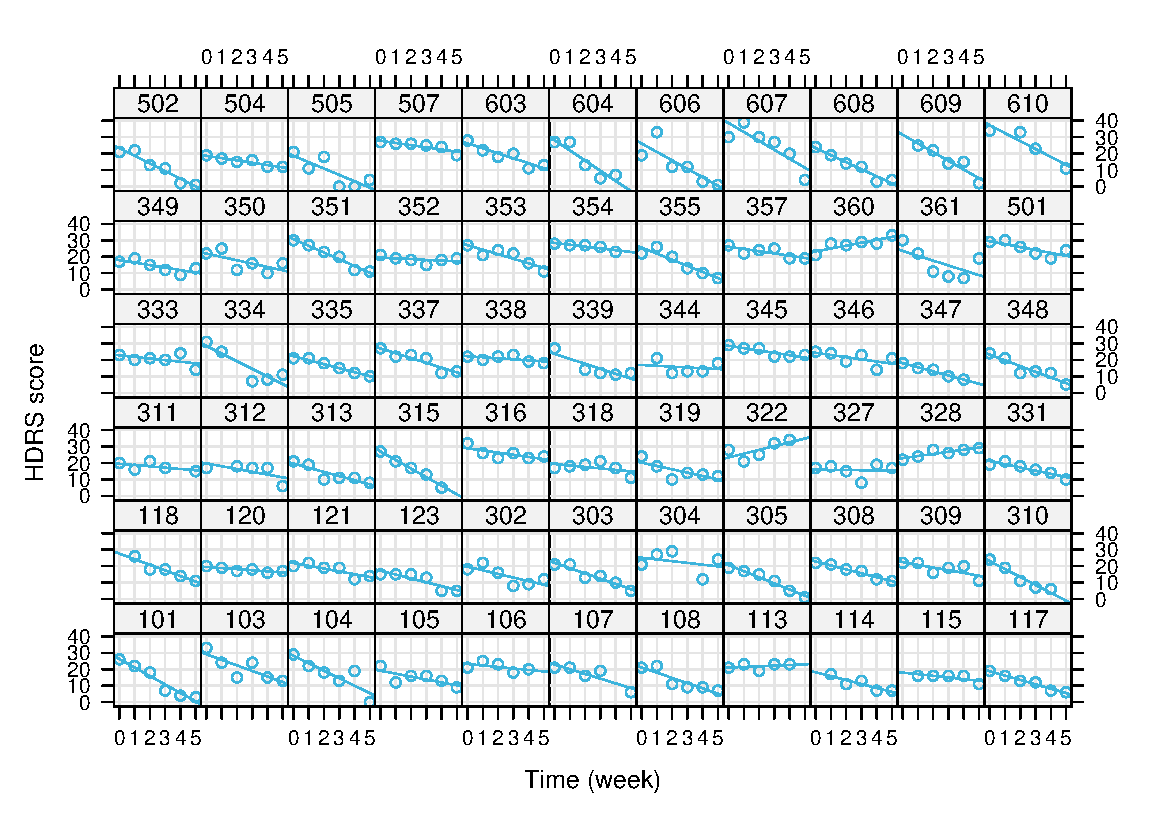
\includegraphics[width=11cm]{figures/hdrs-ind}
\end{column}
\end{columns}
\end{frame}

\begin{frame}{Alternative model with a constant time term}
  \centering
  \vspace{-1cm}
  \[
    y_{ij} = \beta_0 + \beta_1 time + \upsilon_{0i} + \varepsilon_{ij}
  \]
with $\upsilon_{0i} \sim N(0, \sigma^2_{\upsilon})$ i.i.d.,
$\varepsilon_{ij} \sim N(0, \sigma^2)$ i.i.d., $\upsilon_{0i}$ and
$\varepsilon_{ij}$ i.i.d.\\[2ex]
%  with $\varepsilon_{ij} \sim N(0, \sigma_{\varepsilon}^2)$ i.i.d.\ and
%  $\upsilon_{0i} \sim N(0, \sigma_{\upsilon})$ i.i.d.\\~\\

  \begin{tabular}{cccccc}
    \hline
    response & intercept & time effect & time & subject effect  & residual \\
    \hline
    $y_{11}$ & $\beta_0$ & $\beta_1$   & 0    & $\upsilon_{1}$ & $\varepsilon_{11}$ \\
    $y_{12}$ & $\beta_0$ & $\beta_1$   & 1    & $\upsilon_{1}$ & $\varepsilon_{12}$ \\
    $y_{13}$ & $\beta_0$ & $\beta_1$   & 2    & $\upsilon_{1}$ & $\varepsilon_{13}$ \\
    \vdots & \vdots & \vdots   & \vdots & \vdots & \vdots \\
    $y_{21}$ & $\beta_0$ & $\beta_1$   & 0    & $\upsilon_{2}$ & $\varepsilon_{21}$ \\
    $y_{22}$ & $\beta_0$ & $\beta_1$   & 1    & $\upsilon_{2}$ & $\varepsilon_{22}$ \\
    $y_{23}$ & $\beta_0$ & $\beta_1$   & 2    & $\upsilon_{2}$ & $\varepsilon_{23}$ \\
    \vdots & \vdots & \vdots   & \vdots & \vdots & \vdots \\
    $y_{Nn}$ & $\beta_0$ & $\beta_1$   & n    & $\upsilon_{N}$ & $\varepsilon_{Nn}$ \\
    \hline
  \end{tabular}
\end{frame}

\begin{frame}[fragile]{Random intercept model}
  \[
    y_{ij} = \beta_0 + \beta_1 time + \upsilon_{0i} + \varepsilon_{ij}
  \]
with $\upsilon_{0i} \sim N(0, \sigma^2_{\upsilon})$ i.i.d.,
$\varepsilon_{ij} \sim N(0, \sigma^2)$ i.i.d., $\upsilon_{0i}$ and
$\varepsilon_{ij}$ i.i.d.\\[2ex]
\begin{columns}
\begin{column}{6cm}
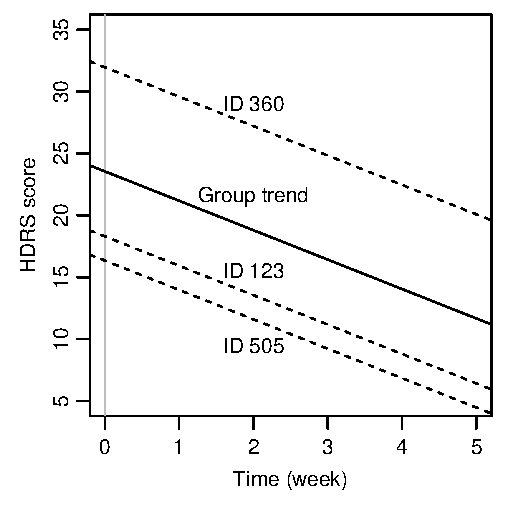
\includegraphics[width=6cm]{figures/hdrs-lme1}
\end{column}
%
\begin{column}{5cm}
  \begin{itemize}
    \item The estimated mean baseline HDRS score is $\hat{\beta}_0 =
      23.55$
    \item However, the estimated standard deviation between patients is
      $\hat{\sigma}_\upsilon = 4.02$
    \item The mean improvement per week is $\hat{\beta}_1 = -2.38$
  \end{itemize}
\end{column}
\end{columns}
% Fitting the mixed-effects model in R
% \begin{lstlisting}[style=plain]
% lme1 <- lmer(hamd ~ week + (1 | id), dat, REML=FALSE)
% \end{lstlisting}
\end{frame}

\begin{frame}{Implied marginal covariance matrix}
  \begin{itemize}
    \item For the three time points $t_{ij} = 0, 1, 2$, $\mat{Z}_i =
      \vect{1}'_{n_i}$ and $\gmat{\Sigma}_\upsilon = \sigma^2_\upsilon$ we
      get
\begin{align*}
  Cov(\vect{y}_i) &=
    \mat{Z}_i \gmat{\Sigma}_\upsilon \mat{Z}'_i + \sigma^2 \mat{I}_{n_i} \\
  &= \sigma^2_\upsilon \vect{1}_{n_i} \vect{1}'_{n_i} +
     \sigma^2 \mat{I}_{n_i} \\
  &= 
  \begin{pmatrix}
    \sigma^2_\upsilon + \sigma^2 & \sigma^2_\upsilon & \sigma^2_\upsilon \\
    \sigma^2_\upsilon & \sigma^2_\upsilon + \sigma^2 & \sigma^2_\upsilon \\
    \sigma^2_\upsilon & \sigma^2_\upsilon & \sigma^2_\upsilon + \sigma^2
  \end{pmatrix}
\end{align*}
\item The random intercept model implies the compound symmetry structure
  \end{itemize}
\end{frame}

% \begin{frame}[fragile]{Random slope model}
%   \[
%     y_{ij} = \beta_0 + \beta_1 time + \upsilon_{0i} + \upsilon_{1i} time +
%     \varepsilon_{ij}
%   \]
% with
% \begin{align*}
%   \begin{pmatrix} \upsilon_{0i}\\ \upsilon_{1i} \end{pmatrix} &\sim
%     N \left(\begin{pmatrix} 0\\ 0 \end{pmatrix}, \, \gmat{\Sigma}_\upsilon =
%       \begin{pmatrix}
%         \sigma^2_{\upsilon_0} & \sigma_{\upsilon_0 \upsilon_1} \\
%         \sigma_{\upsilon_0 \upsilon_1} & \sigma^2_{\upsilon_1} \\
%       \end{pmatrix} \right)
%     \text{ i.i.d.} \\
%   \gvect{\varepsilon}_i &\sim N(\vect{0}, \, \sigma^2 \mat{I}_{n_i})
%     \text{ i.i.d.}
% \end{align*}
% Individual intercepts and slopes each have a unique variance component and
%   correlate with $\varrho_{\upsilon_0 \upsilon_1} =
%   \frac{\sigma_{\upsilon_0 \upsilon_1}}{\sigma_{\upsilon_0} \,
%   \sigma_{\upsilon_1}}$
% 
% % \begin{lstlisting}[style=plain]
% % lme(hamd ~ week + (week | id), dat, REML=FALSE)
% % \end{lstlisting}
% \end{frame}
% 
% 
% \begin{frame}{Model predictions}
% \begin{columns}
% \begin{column}{6cm}
% 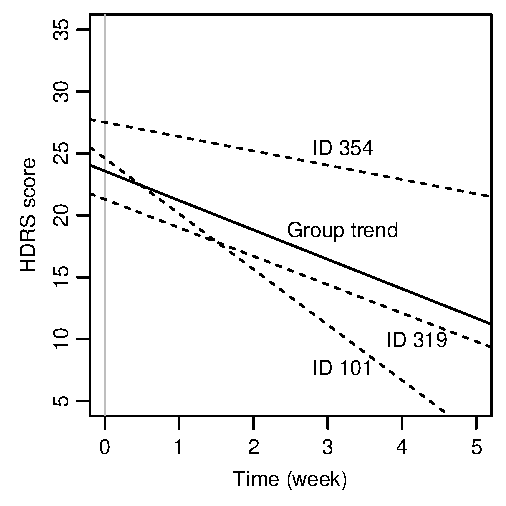
\includegraphics[width=6cm]{figures/hdrs-lme2}
% \end{column}
% %
% \begin{column}{5cm}
%   The estimated mean baseline HDRS score is $\hat{\beta}_0 = 23.58$
% 
%   The estimated standard deviation between patients is
%   $\hat{\sigma}_{\upsilon_0} = 3.55$\\[2ex]
% 
%   The mean improvement per week is $\hat{\beta}_1 = -2.38$
% 
%   The estimated standard deviation between patients is
%   $\hat{\sigma}_{\upsilon_1} = 1.44$\\[2ex]
% \end{column}
% \end{columns}
% The estimated correlation between individual intercepts and slopes is
% $\hat{\varrho}_{\upsilon_0 \upsilon_1} = -0.28$
%   
%   Patients with higher (that means worse) baseline scores improve more
%   strongly than patients with smaller baseline scores
% \end{frame}
% 
% \begin{frame}{Implied marginal covariance matrix}
% For the three time points $t_{ij} = 0, 1, 2$,
% \[
%   \mat{Z}_i =
%     \begin{pmatrix}
%       1 & 0 \\
%       1 & 1 \\
%       1 & 2 \\
%     \end{pmatrix}
%   \text{ und }
%   \gmat{\Sigma}_\upsilon =
%     \begin{pmatrix}
%       \sigma^2_{\upsilon_0} & \sigma_{\upsilon_0 \upsilon_1} \\
%       \sigma_{\upsilon_0 \upsilon_1} & \sigma^2_{\upsilon_1}
%     \end{pmatrix}
% \]
% we get
% \begin{align*}
%   & Cov(\vect{y}_i) =
%     \mat{Z}_i \gmat{\Sigma}_\upsilon \mat{Z}'_i + \sigma^2 \mat{I}_{n_i} \\
%   &= \begin{pmatrix}
%     \sigma^2_{\upsilon_0}                                    & \sigma^2_{\upsilon_0} + \sigma_{\upsilon_0 \upsilon_1}                             & \sigma^2_{\upsilon_0} + 2 \sigma_{\upsilon_0 \upsilon_1} \\
%     \sigma^2_{\upsilon_0} + \sigma_{\upsilon_0 \upsilon_1}   & \sigma^2_{\upsilon_0} + 2 \sigma_{\upsilon_0 \upsilon_1} + \sigma^2_{\upsilon_1}   & \sigma^2_{\upsilon_0} + 3 \sigma_{\upsilon_0 \upsilon_1} + 2 \sigma^2_{\upsilon_1} \\
%     \sigma^2_{\upsilon_0} + 2 \sigma_{\upsilon_0 \upsilon_1} & \sigma^2_{\upsilon_0} + 3 \sigma_{\upsilon_0 \upsilon_1} + 2 \sigma^2_{\upsilon_1} & \sigma^2_{\upsilon_0} + 4 \sigma_{\upsilon_0 \upsilon_1} + 4 \sigma^2_{\upsilon_1} \\
%   \end{pmatrix}
%    + \sigma^2 \mat{I}_{n_i}
% \end{align*}
% hence, a more flexible covariance structure when compared to compound
%   symmetry
% \end{frame}
 
\begin{frame}{Depression and Imipramin: Descriptive statistics}
  {\citep{ReisbyGram77}}
\begin{center}
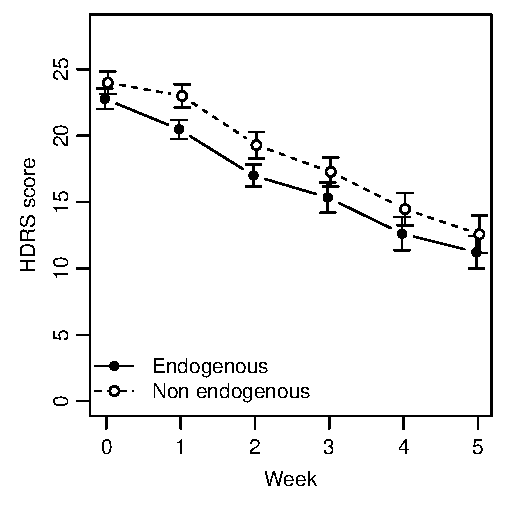
\includegraphics[scale=.8]{figures/hdrs-means-se}
\end{center}
\end{frame}

{\setbeamercolor{background canvas}{bg=iwmgrau!80!white}

\begin{frame}[fragile]{Fitting repeated-measures ANOVA}
  \begin{lstlisting}
# ANOVA with aov()
aov2 <- aov(hamd ~ week2*diag + Error(id/week2),
            dat_val)
summary(aov2)

# Using ezANOVA()
ez2 <- ezANOVA(data = dat_val, dv = hamd, wid = id,
               within = week2, between = diag,
               type = 3)
ez2$ANOVA
  \end{lstlisting}
\end{frame}

\begin{frame}[fragile]{Fitting repeated-measures ANOVA}
  \begin{lstlisting}
# Mixed-effects model
lme2 <- lmer(hamd ~ week2*diag + (1 | id),
            dat_val)
anova(lme2)

# Calculate mean sum of squares for id by hand
sp <- attr(VarCorr(lme2)$id, "stddev")
se <- attr(VarCorr(lme2), "sc")
se^2 + 6*sp^2
  \end{lstlisting}
\end{frame}

\begin{frame}[fragile]{Fitting mixed-effects model}
  \begin{lstlisting}
# And this works on the complete data set
lme3 <- lmer(hamd ~ week2*diag + (1 | id), dat)
anova(lme3)

# Type I sum of squares
m0 <- lmer(hamd ~ 1 + (1 | id), dat, REML=FALSE)
m1 <- lmer(hamd ~ week2 + (1 | id), dat, REML=FALSE)
m2 <- lmer(hamd ~ week2 + diag + (1 | id), dat,
           REML=FALSE)
anova(m0, m1, m2, lme3)
  \end{lstlisting}
\end{frame}

}

\begin{frame}{Repeated measures ANOVA}
  {Two time points}
\begin{itemize}
  \item Regression notation with indicator variable for time ($t_{i1} = 0$,
    $t_{i2} = 1$) and group ($x_i$)
    \[
      y_{ij} = \beta_0 + \beta_1 \, t_{ij} + \beta_2 \, x_i +
               \beta_3 \, (t_{ij} \cdot x_i) + \upsilon_i + \varepsilon_{ij}
    \]
    with $\upsilon_i \sim N(0, \sigma^2_\upsilon)$ and $\varepsilon_{ij}
    \sim N(0, \sigma^2)$
  \item Interpretation
    \begin{center}
    \begin{tabular}{lp{10cm}}
    $\beta_0$ & mean baseline value in reference group\\
    $\beta_1$ & time effect (slope) in reference group\\
    $\beta_2$ & effect of treatment group\\
    $\beta_3$ & effekt on the slope of treatment group
    \end{tabular}
    \end{center}
\end{itemize}
\end{frame}

\begin{frame}{Repeated measures ANOVA}
  {Two time points}
\begin{center}
\begin{tikzpicture}[>=stealth, y=.6cm, x=.6cm, font=\small]
\draw[->] (0,0) -- coordinate (x axis mid) (10,0);
\draw[->] (0,0) -- coordinate (y axis mid) (0,10);
\node[below=0.5cm] at (x axis mid) {Time, $t$};
\node[rotate=90, above=0.5cm] at (y axis mid) {Response, $y$};
%
\draw (3, 4) -- (7, 8) node [above right] {TG};
\draw (4.5, 5.5) -- (5.5, 5.5) -- (5.5, 6) node [right] {$\beta_1 + \beta_3$} -- (5.5, 6.5);
\draw[dashed] (0, 4) node [above right] {$\beta_0 + \beta_2$} -- (3, 4);
%
\draw (3, 2) -- (7, 4) node [above right] {CG};
\draw (4.5, 2.75) -- (5.5, 2.75) -- (5.5, 3.0) node [right] {$\beta_1$} -- (5.5, 3.25);
\draw[dashed] (0, 2) node [above right] {$\beta_0$} -- (3, 2);
%
\draw plot[only marks, mark size=1pt, mark=*]
    coordinates {(3, 4) (7, 8) (3, 2) (7, 4)};
\draw (3, 0.1) -- (3, 0) node [below] {$0$};
\draw (7, 0.1) -- (7, 0) node [below] {$1$};
\end{tikzpicture}
\end{center}
\end{frame}

\begin{frame}{Repeated measures ANOVA}
  {Two time points}
\begin{itemize}
  \item Repeated-measures ANOVA for two time points is equivalent to change
    score analysis
  \begin{itemize}
      \item For the two groups with $j = 1, 2$, we get
        \begin{align*}
          y_{i1} &= \beta_0 + \beta_2 \, x_i + \upsilon_i + \varepsilon_{i1}\\
          y_{i2} &= \beta_0 + \beta_1 + \beta_2 \, x_i + \beta_3 \, x_i + \upsilon_i + \varepsilon_{i2}
        \end{align*}
      \item For the change score, we then get
        \[
          y_{i2} - y_{i1} = \beta_1 + \beta_3 \, x_i + (\varepsilon_{i2} - \varepsilon_{i1})
        \]
      \item Since $\varepsilon_{ij}$ are independent, this results in the
        equation for the change score analysis
        \[
            y_{i2} - y_{i1} = \beta_1 + \beta_3 \, x_i + \varepsilon_{i}
        \]
        with
        \[
            \varepsilon_i = \varepsilon_{i2} - \varepsilon_{i1} \sim N(0, \sigma_d^2 = 2 \sigma^2)
        \]
  \end{itemize}
\end{itemize}
\end{frame}

{\setbeamercolor{background canvas}{bg=iwmgrau!80!white}


\begin{frame}[fragile]{Example: Acupuncture for shoulder pain}
\begin{lstlisting}
# Read data
dat <- read.table("kleinhenz.txt", header=TRUE)
dat$grp <- factor(dat$grp, levels=c("plac", "acu"))

# Change score analysis
m1 <- lm(post ~ offset(pre) + grp, dat)
# Repeated-measures ANOVA
datl <- reshape(dat, direction="long", 
                varying=list(1:2), v.names="score")
datl$time <- factor(datl$time, levels=1:2, 
                    labels=c("pre", "post"))
m2 <- lmer(score ~ grp*time + (1 | id), datl)

# Compare residual variances
sigma(m1)^2
2 * sigma(m2)^2
\end{lstlisting}
\end{frame}

}

% {\setbeamercolor{background canvas}{bg=iwmgrau!80!white}
% 
% \begin{frame}[fragile]{}
%   \begin{lstlisting}
%   ##
%   \end{lstlisting}
% \end{frame}
% 
% }
% 
% \begin{frame}[fragile]{}
%   \begin{block}{Exercise}
%     \begin{itemize}
%       \item 
%     \end{itemize}
%   \end{block}
% \end{frame}

\appendix
%\begin{frame}[allowframebreaks]{References}
\begin{frame}{References}
%\renewcommand{\bibfont}{\footnotesize}
\bibliographystyle{apacite}
\bibliography{../../../literature/nu}
\vfill
\end{frame}

\end{document}

